\section{Interface graphique}\label{interface}

Notre interface graphique est construite avec GTK+ 2.0 et s'organise de 
la manière suivante:

\begin{itemize}
    \item Une fenêtre principale contenant:
    \begin{itemize}
        \item Une barre de menu pour accéder aux fonctionnalités 
        (nouvelle partie, niveau de difficulté, scores, etc.)
        \item Une zone d'information montrant les prochaines boules et le score actuel
        \item La grille de jeu, composée de boutons représentant les cases
    \end{itemize}
\end{itemize}

\begin{figure}[H]
    \centering
    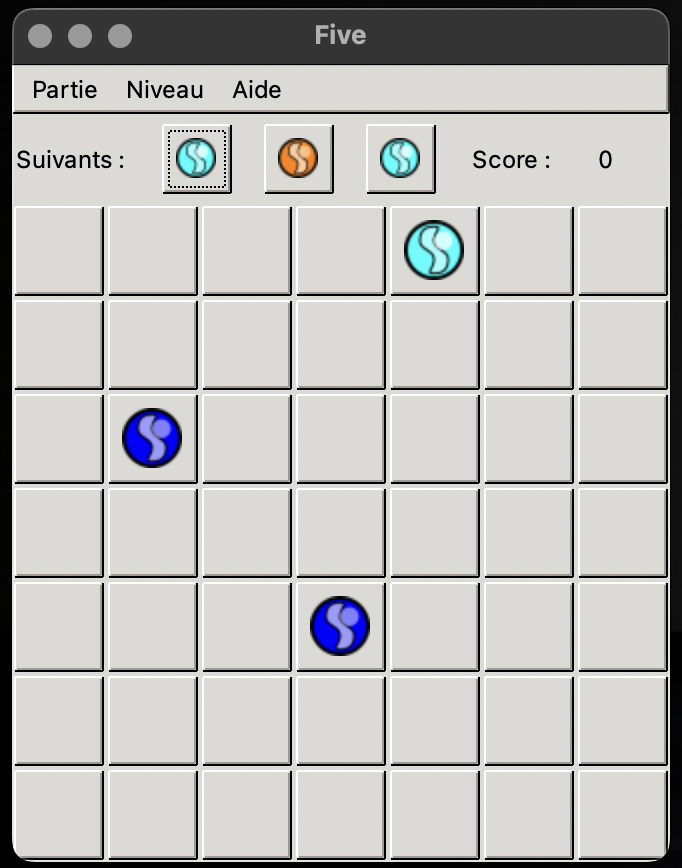
\includegraphics[width=0.4\textwidth]{interface.jpeg}
    \caption{Interface du jeu Five or More}
    \label{fig:Interface}
\end{figure}

La fenêtre est organisée avec des widgets GTK imbriqués:
\begin{itemize}
    \item La fenêtre principale contient une VBox verticale
    \item Dans cette VBox, nous avons placé:
    \begin{itemize}
        \item La barre de menu (GTK MenuBar)
        \item Une HBox horizontale pour les prochaines boules et le score
        \item Une Table GTK pour la grille de jeu, dont la taille varie selon 
        le niveau de difficulté
    \end{itemize}
\end{itemize}

Nous avons dû utiliser GtkTable pour cela. 
Chaque case du jeu est représentée par un GtkButton pouvant contenir une image 
de boule grâce à notre fonction: \\
$GtkWidget ${ }$ *charger\_image\_button(const ${ }$ char { } *chemin\_image)$
